\chapter{Design Motivation}
\label{ch:fddp-design}

%%%%%%%%%%%%%%%%%%%%%%%%%%%%%%%%%%%%%%%%%%%%%%%%%%%%%%%%%%%%%%%%%%%%
\section{Introduction to Dual-Phase Far Detector in DUNE}
\label{sec:fddp-design-highlight}


The DUNE dual-phase LArTPC detector design 
has a fully homogeneous liquid argon volume, in which electrons
drift upwards vertically towards an extraction grid just below the liquid-vapor interface. From there they
are extracted from the liquid into the gas phase, amplified, and
collected on a finely segmented
anode.


\begin{dunefigure}[optional caption for LoF]{fig:figure-label-DPprinciple}
{required full caption (Credit: xyz)}
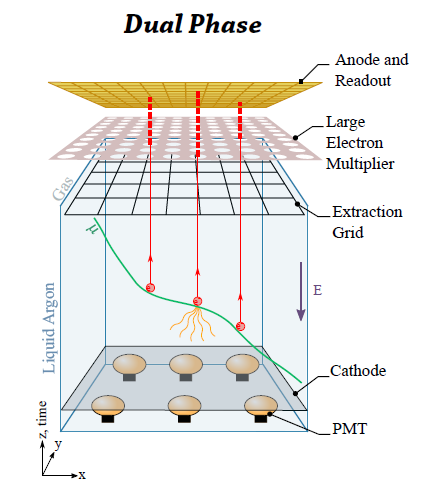
\includegraphics[width=0.6\textwidth]{dualphase-principle}
\end{dunefigure}

The electron amplification in the gas phase enables a robust and tunable signal-to-noise ratio. 
The detector configuration is similar to a single-phase LArTPC. The features of the dual-phase design, e.g., high gain, 
allow achieving very long drift paths and large detector dimensions while minimizing the number of readout channels.


This innovative dual-phase design is similar in many ways to the single-phase design,
but implements some unique features and offers several advantages over it, in particular
\begin{itemize}
\item  higher gain, leading to a larger signal-to-noise ratio (S/N);
\item  larger fiducial volume, enabling very long drift paths;
\item  lower detection threshold;
\item  finer readout pitch (3~mm), implemented in two identical collection views, $x$ and $y$;
\item  fewer readout channels (153,600 vs 384,000 for a reference design \ktadj{10} module); and
\item  the absence of dead material in the LAr volume.
\end{itemize}

